\documentclass[lettersize,journal]{IEEEtran}
\usepackage{amsmath,amsfonts}
\usepackage{algorithmic}
\usepackage{algorithm}
\usepackage{array}
\usepackage[caption=false,font=normalsize,labelfont=sf,textfont=sf]{subfig}
\usepackage{textcomp}
\usepackage{stfloats}
\usepackage{url}
\usepackage{verbatim}
\usepackage{graphicx}
\usepackage{cite}
\usepackage{color}
\usepackage{ulem}	
\hyphenation{op-tical net-works semi-conduc-tor IEEE-Xplore}

% updated with editorial comments 8/9/2021

\begin{document}

\title{A Selective Bit Dropping and Encoding Co-Strategy  in Image Processing for Low-Power Design in DRAM and SRAM}
%,Kaitong Zhang,Qingyang Yu,Lingxiao Yan,Tong Wang,Jin Yu,Ni Zhou
\author{~\IEEEmembership{Mingkai Liu, Haohua Que, Xinghua Yang, Kaitong Zhang, Qingyang Yu, Lingxiao Yan, Tong Wang, \\ Yu Jin, and Ni Zhou}
%\thanks{This work was supported by the Fundamental Research Funds for the Central Universities under Grant No.BLX202015 and Beijing
%Municipal Natural Science Foundation under Grant No.6222038.}% <-this % stops a space
\thanks{Mingkai Liu, Haohua Que, Xinghua Yang, Qingyang Yu, Lingxiao Yan, Tong Wang and Yu Jin are with Electronics and Information Technology Department, Beijing Forestry University, China 100091.}
% (e-mail:KleinKai565@bjfu.edu.cn; qh13005968844@bjfu.edu.cn; yangxh@bjfu.edu.cn; yuqingyang001@bjfu.edu.cn; Yanlx4869@@bjfu.edu.cn; WangTom@bjfu.edu.cn; AUH2OJin@bjfu.edu.cn).
\thanks{Kaitong Zhang is with Vehicle Engineering Department, Beijing Forestry University, China 100091. }
\thanks{Ni Zhou is with Electronic Engineering Department, Tsinghua University, China 100091.}
\thanks{Mingkai Liu, Haohua Que contributed equally to this work and be considered co-first authors.}
\thanks{Xing-Hua Yang is the corresponding author.}
}

% The paper headers
\markboth{Journal of \LaTeX\ Class Files,~Vol.~14, No.~8, August~2021}%
{Shell \MakeLowercase{\textit{et al.}}: A Sample Article Using IEEEtran.cls for IEEE Journals}

%\IEEEpubid{0000--0000/00\$00.00~\copyright~2021 IEEE}
% Remember, if you use this you must call \IEEEpubidadjcol in the second
% column for its text to clear the IEEEpubid mark.

\maketitle
\begin{abstract}
 A novel and efficient way of image processing is proposed  in this paper, which fully exploits the features of DRAM (Dynamic Random Access Memory) and SRAM (Static Random Access Memory) as well as the human visual system. The proposed  strategy first approximates and encodes the image  to  effectively reduce the number of bit-`1' in the original pixel data,  then the processed data is pushed into the off-chip DRAM, and later written into the on-chip SRAM for further computation. Since the storage power consumption of DRAM is proportional to the number of bit-`1', while the write power consumption of SRAM is linear relative to the switch probability and the square of the supply voltage,  fewer bits-`1'  in the processed pixel data will decrease  the power consumption of DRAM and SRAM, yet accompanied by negligible influence on output quality as our proposed method has the advantages of both approximate computation and error compensation. Thus, a tradeoff is finally achieved between storage power consumption and output quality. \textcolor{red}{The recommended strategy has been implemented in digital circuits, and the algorithm complexity is not increased by embedding the proposed scheme into the integrated image processing algorithm and the system modification is negligible.} In the experimental simulations, 39.8\% power reduction for DRAM and 25.9\% write power reduction for SRAM have been achieved. Regarding output quality, Discrete Cosine Transform (DCT), quantization, inverse quantization and inverse DCT (IDCT) are employed to process the approximated data. The simulations shows \textcolor{red}{average} 3.36 dB losses in Peak-Signal-Noise-Ratio(PSNR). Based on this strategy, an approach of priority-based reduction in supply voltage for insignificant pixel data is introduced to achieve further reduction in power consumption for SRAM. Undoubtedly, a lower supply voltage will increase the probability of read errors from SRAM. However, with our proposed approximate coding strategy, the output quality is barely impacted by the lower supply voltage. 
\end{abstract}

\begin{IEEEkeywords}
Approximate storage, embedded system, DRAM, SRAM, image processing, low power design.
\end{IEEEkeywords}

\section{Introduction}
\IEEEPARstart{W}{ith} the large-scale application and development of new computer vision and artificial intelligence in recent years, applications like high-definition images and videos are gradually being ported to embedded devices such as mobile phones, tablets and wearable devices. As a result, there are higher demands on the computation and storage of large-scale data, especially in storage as it accounts for more than 90\% of the power consumption \cite{7560228,culler1999parallel} in common image and video applications. The storage power consumption is generally divided into two parts: off-chip storage DRAM and on-chip storage SRAM. In typical image processing, as shown in Fig. \ref{fig1}, the raw image data will first be sent to off-chip storage DRAM, followed by on-chip SRAM for further computation, and some outputs of the computation will be sent back to DRAM. Due to battery capacity and the slow development of new storage materials, reducing the power consumption of DRAM and SRAM storage in existing embedded systems is a serious concern.
\begin{figure}[htb]
\centering
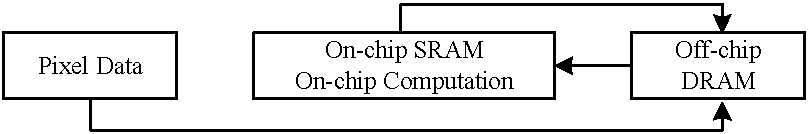
\includegraphics[width=\linewidth]{Fig/Dataflow of typical image processing.png}
\caption{Dataflow of typical image processing.}
\label{fig1}
\end{figure}

Lowering the amount of image data is one of the normal ideas for reducing storage power. The most well-known approach is image compression \cite{4607562}, which implements a compression algorithm to decrease the amount of image data before  transferred and stored in the off-chip storage DRAM. However, this approach has two major defects: firstly, compression algorithm is complex to implement, such as adaptive bit-width compression \cite{1435140}, a dictionary-based fixed length coding scheme \cite{4590164}, especially considering the power consumption of embedded devices is limited; Secondly, the system modification and overhead required to integrate the compression algorithm into the existing image and video processing system are significant.

A different idea is to build on existing algorithms to reduce power consumption by changing the storage structure, or by preprocessing the raw image data. \textcolor{red}{For example, the 8T structure of SRAM proposed by Dr. Mohapatra \cite{5686921} changes the storage structure at the transistor level, and the designer needs to redesign the layout so that the new storage structure can be practically applied in the integrated circuit, which brings additional expenses that are not acceptable for practical applications. As for the preprocessing methods, s}ome of the common solutions include data encoding \textcolor{red}{and} data dropping {\color{red}\sout{and supply voltage reduction, etc.}} In contrast to precisely computed circuit systems, image and video processing takes advantage of the fact that the human visual system is more sensitive to low frequency than high frequency \cite{wang2002video,7153874}. For example, during the common lossy decompression of JPEG images, the human eye is comparably less sensitive in distinguishing the results of output  when the PSNR is above 30 dB. In other words, a completed accurate storage method is not necessary in practical applications. Therefore, the data in storage system can be divided into important and non-important parts depending on the perceptual sensitivity of the human eye. More specifically, for a pixel value, the information in the high-bit part is more crucial than those in the low-bit part \cite{5523464}. Based on this feature, through exploring the characteristics of DRAM and SRAM, the pixel data can be selectively approximated or encoded in advance in order to provide a corresponding solution to reduce storage power consumption. 

This paper proposed a method for preprocessing raw image data with selective bit dropping and approximate encoding strategies, as well as an approach of priority-based reduction in supply voltage for insignificant pixel data to achieve further reduction in power consumption. The proposed data could preserve the most significant information of the image data effectively, and has a limited impact on output quality. A tradeoff has been achieved between power savings and output quality as 39.8\% power reduction for DRAM and 25.9\% write power reduction for SRAM are shown in the extensive simulations, with only 3.36 dB  losses in PSNR compared to accurate processing. The technique for lowering supply voltage for insignificant pixel data can be used in addition to the strategy to reduce storage power consumption. The results from the subsequent experimental data demonstrated that it has a {\color{red}\sout{negligible}} \textcolor{red}{surprising} effect on output quality.

The structure of the paper is as follows: Section \ref{sec2} gives an introduction of SRAM and DRAM. The proposed strategy is described in Section \ref{sec3}. Section \ref{sec4} presents the experiment results. The paper is concluded in the final section.
\begin{figure*}[htb]
\centering
\subfloat[]{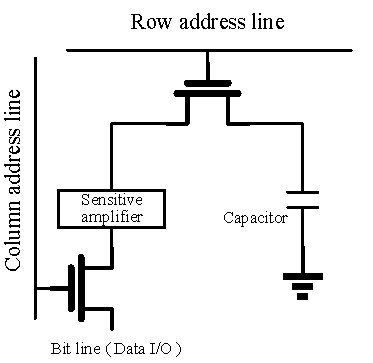
\includegraphics[width=.4\linewidth]{Fig/(a) circuit scheme of one bitcell in DRAM.png}}
\hfil
\subfloat[]{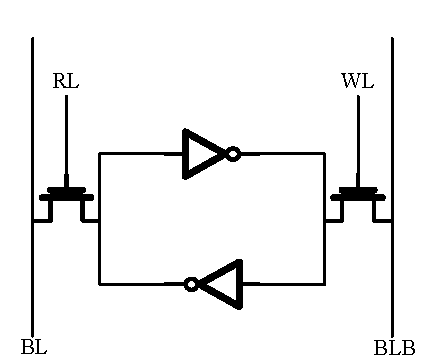
\includegraphics[width=.4\linewidth]{Fig/(b) circuit scheme of one bitcell in SRAM.png}}
\caption{Circuit scheme of bitcell in DRAM and SRAM. (a) circuit scheme of one bitcell in DRAM. (b) circuit scheme of one bitcell in SRAM.}
\label{fig2}
\end{figure*}

\section{Power Analysis of SRAM and DRAM} \label{sec2}
Both DRAM and SRAM account for a large percentage of the power overhead in circuit systems, where the read/write and refresh operations consume the most of the power consumption for DRAM and SRAM. Fig. \ref{fig2}(a) \cite{5741318} shows the basic cell of a single-bit DRAM, which is composed of three basic modules: two NMOS transistors, a sensitive amplifier and a capacitor to store data. When the read/write operation is performed, the row address line and column address line are first activated to ``1", and the NMOS transistors are turned on. The sensitive amplifier is then used to connect the bit line to the capacitor. When the data is ``1" or ``0", the capacitor will be charged and discharged according to the read/write operation. It should be noted that when the data is stored as ``1", the charge stored on the capacitor will deplete over time due to the capacitor’s leakage current, so the entire DRAM needs to be dynamically refreshed in regular intervals to replenish the leaked charge to ensure the accuracy of the stored data. While no charge replenishment is required during the refresh process if the original stored data is ``0", i.e. no additional dynamic power consumption is generated when the data is stored as ``0". Therefore, as stated in \cite{10.1145/513918.514138,5741318}, the storage power consumption of DRAM is proportional to the number of bit-`1'. In order to reduce the storage power of DRAM, Dr. Song et al. \cite{10.1145/1961296.1950391} proposed a multi-level refresh frequency for approximate storage. Likewise, the authors kept the refresh frequency of the significant bits constant and reduced the refresh frequency of the insignificant bits to varying degrees based on the principle that the high bits of the original image data cannot be contaminated and the low bits can be approximated. The main problem with this approach is the need to modify the original DRAM refresh control system. It is impossible to ignore the additional overhead caused by this modification process. Moreover, approximate storage with complete bit dropping method for original stored data to decrease the power consumption of off-chip DRAM is a common approach. Nevertheless, complete bit dropping method could generate excessive loss of raw data information and require real-time dynamic monitoring of the output quality \cite{miao2014modeling}. In this context, data encoding from \cite{10.1145/605459.605464} proposed an efficient approach to reducing the number of bit-`1' for DRAM storage. However, bandwidth utilization is a key problem due to additional flags and information.

Compared with DRAM, the storage process of SRAM is relatively simple. The power consumption of SRAM can be divided into three parts: write power, read power and leakage power. Fig. \ref{fig2}(b) \cite{5686921} shows the basic cell of a single-bit SRAM. This single-bit memory structure consists of 6 MOS transistors (6T structure), where the two inverters in the middle constitute the positive feedback while the two NMOS transistors on both sides serve as the write and read interfaces of the memory cell. When the write operation is performed, the WL and RL are first activated to ``1", and the two NMOS transistors are turned on. Through the BL, BLB and the two NMOS transistors, the input data will be written into the inverters. Two situations occur in this case. If the written data is opposite to the currently saved data, the intermediate inverters with positive feedback loop will be forcibly flipped to the desired value, during which both inverters are charged, discharged and consume energy. The write operation will not generate flipped power if the data value being written matches the data value kept in the prior state. As for read power and leakage power, \cite{5686921,4342716} pointed out that the value of write power is 3.3X larger than that of read power, and the leakage power consumption is only a small fraction of SRAM power dissipation. In summary, data write power is the main source of power consumption for on-chip SRAM. More specifically, most of the power consumption occurs when the transistors of the bit-cell in SRAM switch between the on and off state. Therefore, lots of research has been done in the past to reduce write power consumption. For the on-chip memory cell circuit, the energy overhead is proportional to several parameters as shown in Eq. \eqref{equ1}:
\begin{equation}
\label{equ1}
\boldsymbol{E}\propto \boldsymbol{\alpha CV}_{\boldsymbol{DD}}^{2}\boldsymbol{f}
\end{equation}

Where $\boldsymbol{E}$ is the energy overhead, $\boldsymbol{\alpha}$ is the switch probability (switches between bit-`1' and bit-`0'), $\boldsymbol{C}$ is the effective capacitance, $\boldsymbol{V}_{\boldsymbol{DD}}$ is the supply voltage and $\boldsymbol{f}$ is the operating frequency \cite{6387646}. In a practical circuit design, the circuit equivalent capacitance is mainly related to the circuit structure, and it is extremely complicated to improve from the design. Although reducing the operating frequency may seem effective for large-scale data operations, this will reduce the circuit’s performance as there is no guarantee of real-time data processing in the circuit system \cite{6152179}, which is unacceptable in practical image processing applications. Since energy has a squared relationship with supply voltage, reducing the voltage is an effective method \cite{6409436}. However, when reducing the supply voltage, the circuit’s ability to run at a high frequency decreases and the susceptibility to circuit noise increases. The circuit will have timing errors if the operating frequency is forced to be constant. In short, lowering the supply voltage may result in an incorrect circuit's logic output. A mixed approximate storage scheme can therefore be adopted in light of the fact that the high bits of the original image data cannot be contaminated and the low bits can be approximated. The normal supply voltage can be used for the important part of the pixel data, while the lower supply voltage can be applied for non-important part. Moreover, since SRAM write power consumption is proportional to the switch probability, reducing the $\boldsymbol{\alpha}$ value in Eq. \eqref{equ1} is also considered an efficient way to achieve power consumption.

From the analysis above, reducing the number of `1' is critical for saving DRAM power consumption, whereas decreasing the switch probability $\boldsymbol{\alpha}$ in Eq. \eqref{equ1} is an effective approach that can also be utilized jointly with a mixed voltage approximate storage scheme for saving power consumption of SRAM.


%From the analysis above, reducing the number of `1' is critical for saving DRAM power consumption, whereas decreasing the switch probability $\boldsymbol{\alpha}$ in Eq. \eqref{equ1} is an effective approach that can also be utilized jointly with a mixed voltage approximate storage scheme for saving power consumption of SRAM.


\section{Co-Strategy of Selective Bit Dropping and Encoding with Supply Voltage Reduction } \label{sec3}


{\color{red}\subsection{The proposed Co-strategy}}
As previously indicated, the power consumption of DRAM could be effectively reduced if most of the bits stored in the original image are bit-`0'. More crucially, the probability of switching in the entire SRAM write operation is simultaneously reduced when the image data with this feature is cached from off-chip DRAM to on-chip SRAM for further computation. Therefore, SRAM’s storage power consumption can also be effectively reduced. Thus, we can focus on the preprocessing of original image data and no more design overhead or large modification to the circuit system are needed. The encoding and complete bit dropping mentioned above are two effective methods to reduce the number of bit-`1' in the raw image data. However, the encoding method introduces additional flags, reducing the bandwidth availability of off-chip storage significantly. Meanwhile, complete bit dropping method leads to excessive data losses. In this paper, we try to optimize both methods and combine the results to obtain our approximate storage method. The proposed method is as follows:

Based on the fault tolerance of image video, \textcolor{red}{the least significant bit} {\color{red}\sout{the last bit of a pixel value}} \textcolor{red}{(LSB)} {\color{red}\sout{(8 bits per pixel as illustrated)}} is used as the encoding flag bit, which means that we do not introduce extra bit-flags. Our initial focus is on the high seven bits of the pixel data. From high to low order, the high seven bits are designated as $bit_7$, $bit_6$, $bit_5$, $bit_4$, $bit_3$, $bit_2$, and $bit_1$. These seven bits are divided into two parts: the high part, which is from $bit_7$ to $bit_{_{8-K}}$, and the low part, which is from $bit_{_{7-K}}$ to $bit_1$, $K \in [1,7]$. $K$ value denotes the number of pixel bits in the high part. In the case of $K$ = 7, the number of pixel bits in the low part is 0. When $K$ = 1, the number of pixel bits in the high part is 1, and the number of pixel bits in the low part is 6.


After capturing the raw data of the image, as the low bits in the pixel data are insignificant, for the low part bits, which is from $bit_{_{7-K}}$ to $bit_1$ ($K \in [1,7]$), we proposed an approximate compensation dropping method to keep the first bit- `1' from high order to low order in $bit_{_{7-K}}$ to $bit_1$, and then set the other bits to zero. Unlike the complete dropping method, this method retains the highest bit with logical value `1' and provides various degrees of error compensation for different degrees of data approximation. When the number of dropped bits is higher, this method will be more advantageous. Since more bits in low part of the pixel will be set to zero, the power consumption of DRAM could be reduced effectively. Moreover, the switch probability $\boldsymbol{\alpha}$ in Eq. \eqref{equ1} could also be reduce to achieve further power savings in SRAM.


Simultaneously, as high bits are important in pixel data, the original data must be stored accurately. A flip encoding method is proposed here to reduce the number of bit-`1' in the high part. Fig. \ref{fig3} shows the proposed encoding scheme. First, the number of bit- `1' in the high part is counted. When the number of bit- `1' is greater than $K$/2, all the bits in the high part are flipped, and the flag bit({\color{red}\sout{the last bit of the pixel}} \textcolor{red}{LSB} as we described before) is enforced as `0'. When the number of bit- `1' is smaller than $K$/2, the data in the high part remains unchanged with the flag bit will be set as `1'. Using {\color{red}\sout{the}} \textcolor{red}{LSB} {\color{red}\sout{last bit}} as the flag information has no effect on the bit width of the data. Instead, it can effectively reduce the number of bit-`1' in the high part. The flag bit is utilized to determine whether to flip the high part during the decoding operation. If it is `0', then flip it; if it is `1', keep it constant. This simple-to-implement and easy-to-integrate \textcolor{red}{encoding and} decoding operation does not modify the current image decoding system, making it an efficient method to reduce the number of bit-`1'.
\begin{figure}[htb]
	\centering
	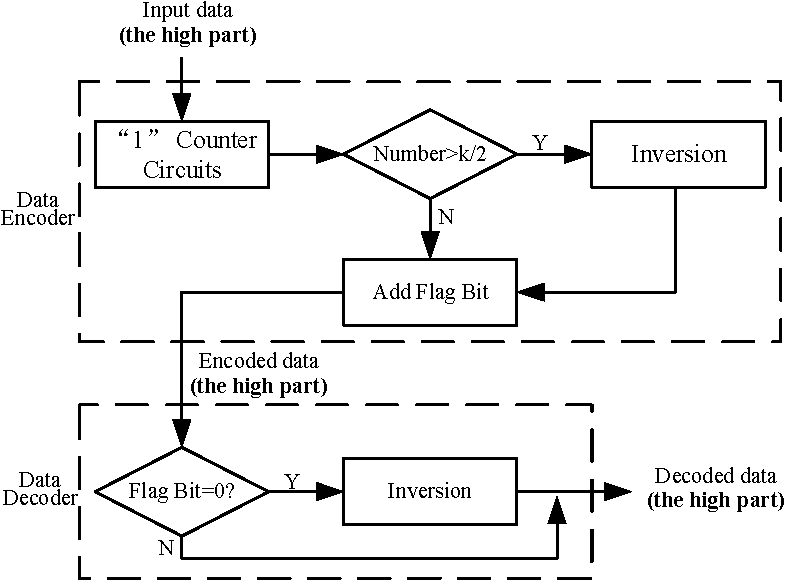
\includegraphics[width=\linewidth]{Fig/Encoding scheme for the high part.png}
	\caption{Encoding scheme for the high part.}
	\label{fig3}
\end{figure}


As illustrated in Fig. \ref{fig4}, with $K$ = 4 as an example, the high part contains four bits from $bit_7$ to $bit_4$ and the low part contains three bits from $bit_3$ to $bit_1$. As shown in the diagram, if the number of bit-`1' is greater than 2, it will be flipped and the corresponding flag bit is set to `0'. If the number of `1' is less than or equal to 2, the flip will not occur and the corresponding flag bit will be set to `1'. As for the low part, it is clear that the data after the first bit-`1' position is cleared.
\begin{figure}[htb]
	\centering
	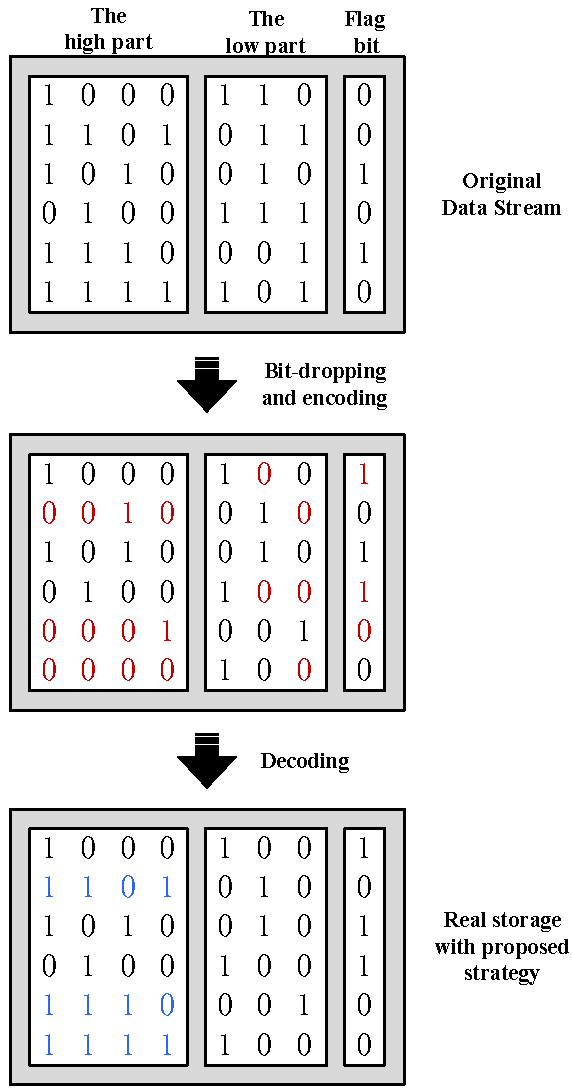
\includegraphics[width=.75\linewidth]{Fig/Illustration of the proposed strategy.png}
	\caption{Illustration of the proposed strategy.}
	\label{fig4}
\end{figure}

It can be seen that with smaller value $K$, more bits will be assigned to the low part, which means that more bits could be set to bit-`0' to achieve power savings. Meanwhile, the larger amount of bit-`0' in the low part of the pixel data indicates that more information will be lost in the image, resulting in poor output quality. However, it should be noted that the output quality requirements for image processing during real-world applications are various. As shown in Fig. \ref{fig5}, the designer can set an output quality threshold for a specific image application. 
\textcolor{red}{To meet different requirements for output quality in different applications, the hardware designers should implement the Co-strategy proposed herein through the high-level language of C/C++ before starting their design. When the original data is collected by the image acquisition device, the value of k should be taken from 7, and the original data should be put into the simulated Co-strategy for approximation storage processing. With the decline of the k value, the output quality will be judged successively in the test process to determine whether it meets the requirements of different designers. For varying processing algorithms, different parameters can be selected to check the output quality. }
For example, PSNR is a common output quality evaluation index that could adjust the size of the $K$ value to determine whether the output quality threshold is satisfied. The minimum value of $K$ is obtained if the output quality threshold is satisfied, so as to obtain the minimum storage power consumption. It should be noted that if the output $K$ value of Fig. \ref{fig5} is 8, which is outside the range of $K$, the output quality requirement cannot be met when $K$ = 7. At this point, accurate processing should be taken and no data preprocessing can be done. If the output $K$ value is 0, which is also outside the range of $K$, it is clear from the above analysis that the number of bits in the high part is 0, the encoding scheme will be ignored, and as a result the resources of the flag bit are wasted.
\textcolor{red}{What also needs to be noted is that, when $K=7$, the number of bits in the high part is 7, and the number of bits in the low part is 0. This means that only the encoding method works. When $K=6$, the number of bits in the low part is 1. In this occasion, the original value of the logic value of this bit will be reserved due to the features of the data-compensated dropping method. Therefore, actually the method of data-compensated dropping will fail to work either; meanwhile, the number of bits in the higher part is 6, which is one bit less than that of $K=7$. This implies that the number of bits participating in the encoding method is one bit less, so the power consumption rises accordingly compared with that of $K=7$. The features when $K=6$ will be confirmed in the subsequent experiments. Thus, the designer should be aware that, when $K=6$, $K=7$ should be the better choice.}
 \begin{figure}[htb]
 	\centering
 	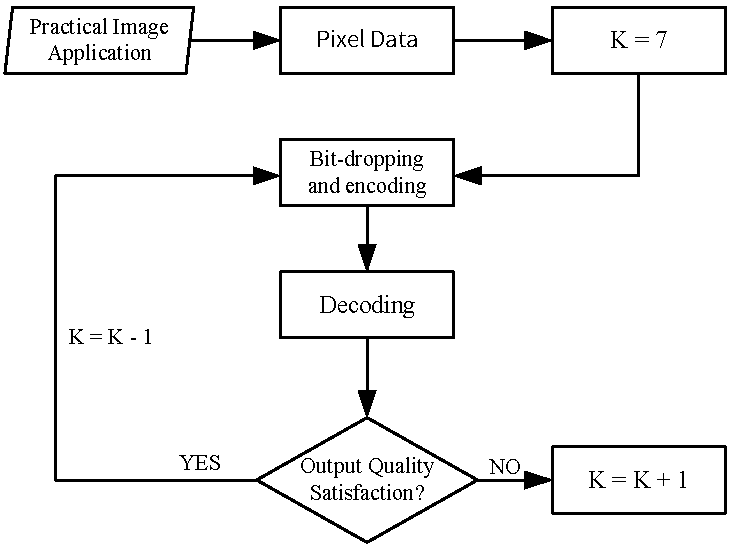
\includegraphics[width=\linewidth]{Fig/Proposed data analysis method.png}
 	\caption{Proposed data analysis method.}
 	\label{fig5}
 \end{figure}

{\color{red}\subsection{The implementation of integration}}

\textcolor{red}{The method of merging the error compensation dropping method with the encoding method is proposed herein. After determining the k value, for the implementation of specific hardware the hardware designer needs to consider the implementation of both methods.}

\textcolor{red}{For the error-compensated dropping method, each pixel needs to be pre-processed by a dedicated digital circuit, and the basic digital gate should be employed. Taking k=4 as an example, its logic computation structure is as shown in Fig. a.}

\textcolor{red}{Where $P_{original}[7 : 0]$ is the input data of a single pixel, while $P_{approximate}[7 : 0]$ is the approximate data after pre-processing. $P[7]$ represents the most significant bit (MSB) of the pixel data. Therefore, the following bits from high to low are $P[6]$, $P[5]$, $P[4]$, $P[3]$, $P[2]$, $P[1]$, and $P[0]$. When $K=4$, the original logic values of 4 bits in the high part and LSB (as flag information) are directly copied, and the three bits in the low part need to be processed by the error-compensated dropping method. According to the proposed pre-processing algorithm, $P[3]$ is the highest bit of the approximate storage. If $P[3]$ is logic `1', it needs to be retained; but if it is logic `0', the logic value of $P[2]$ needs to be observed further. Therefore, in terms of logic computation, the assignment of $P[3]$ comes directly from the original data. When P[3] logic is `0', the logic value of $P[2]$ needs to be considered. If $P[2]$ is logic `1', it needs to be retained; but if it is logic `0', the logic value of $P[1]$ needs to be observed further. The subsequent bits should be processed similarly until the last bit of the low part. Therefore, the whole process contains a series of ``NOT'' gates and ``AND'' gates logic computation. It is evident that the whole computation process can be implemented through a few simple logic gates.} 

\textcolor{red}{Fig. b demonstrates the implementation of this method in the MPEG-2 decoding system [9]: it is inserted between the SDRAM controller and the MPEG-2 decoder core. No additional decoding costs are needed on the control scheme for parts connected to data encoders and decoders, such as Ref.picture reading, VGA display controllers, etc. Since the modification of the original modules is unnecessary, the time series and control of the decoding system remain unaffected. This indicates that the method can be easily implemented, and rapidly and efficiently integrated into a video decoding system.}

\textcolor{red}{From the above analysis, the logic design of the error-compensated dropping method and the encoding method is simple and they can be easily coded in Verilog and synthesized by DesignCompiler tools. In addition, according to the following simulations, the circuit overload brought by these two methods is negligible. More importantly, the pre-processed circuit can be embedded into the image and video processing algorithm conveniently. The system modification brought therefrom is negligible.}


Based on the above analysis, it is clear that the proposed method could achieve the tradeoff between storage power consumption and output quality while being more efficient than the approaches previously mentioned. As the method focuses solely on image data preprocessing, the storage structure is not modified and the method is simple to implement, requiring no system modifications. More importantly, the strategy can also be utilized in conjunction with an approximate mixed voltage storage scheme. The read errors from SRAM due to the reduced supply voltage could ``recover" the missing pixel information. The result will be demonstrated in later simulations.

\section{Experimental simulations} \label{sec4}

In this section, the proposed strategy is modeled through C++. As shown in Fig. \ref{fig6}, the pixel data are preprocessed with different approximations using different $K$ values. According to the typical data flow process in image processing applications, the processed pixel data is pushed into DRAM and SRAM, where the number of bit-`1' per pixel for storage in DRAM and the switch probability for storage in SRAM are simulated and analyzed. In terms of output quality, the preprocessed pixel data is first decoded before being pushed into the simulation of the common JPEG and MPEG-2 codec core algorithms, and the PSNR value of the final output image is used as a metric for output quality.
\begin{figure}[htb]
	\centering
	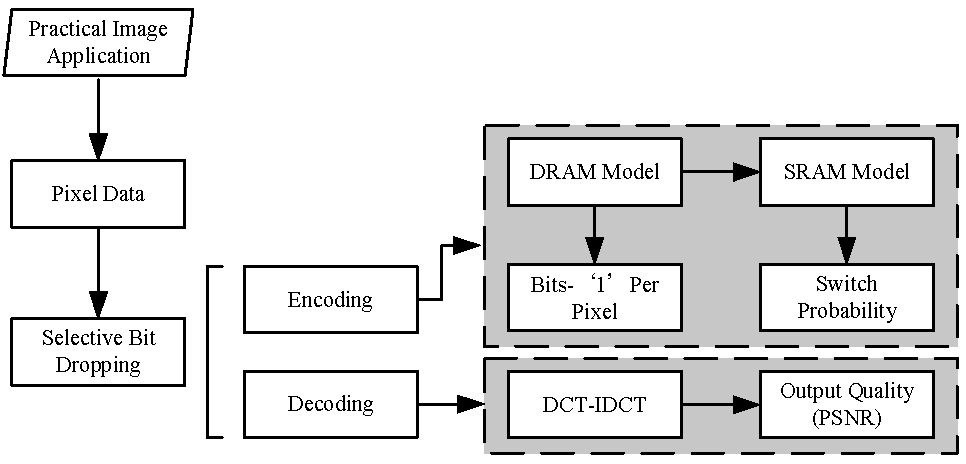
\includegraphics[width=\linewidth]{Fig/Flow chart for experimental simulation.png}
	\caption{Flow chart for experimental simulation.}
	\label{fig6}
\end{figure}

\subsection{Simulation results for the number of bit-`1' in DRAM and the switch probability in SRAM}

{\color{red}\sout{Since the image preprocessing does not change the off-chip and on-chip memory systems and image processing algorithms, it can be easily integrated into the front end of the image processing algorithm.}} The image preprocessing algorithm including selective bit dropping and encoding has been implemented in C++. After preprocessing with different values of $K$, real image data featuring a resolution of 256*256 is sent to the DRAM model, and the simulation result of storage power consumption in DRAM is shown in Fig. \ref{fig7}. {\color{red}\sout{The measure of storage power consumption is the average number of bit-`1' per pixel}} Navg \textcolor{red}{refers to the average number of bit-`1' per pixel (as the measure of storage power consumption in DRAM)}. The pixel data without preprocessing, i.e., the accurate storage method, is used as the baseline for comparison with the approximate preprocessing method. It can be seen that Navg {\color{red}\sout{in DRAM}} for yet-to-be-preprocessed pixel data is 4.22, which is close to 50\%. When $K=7$, only the flag bit (as the encoded flag information) at the end of the pixel data is lost, but Navg decreases to 2.81, reducing the DRAM storage power consumption by 33.4\%. This shows the efficiency and effectiveness of the encoding scheme. More notably, if the requirement for the output quality is not so high, the value of $K$ can be reduced even further. As illustrated in the analysis above, the value of Navg decreases significantly as $K$ decreases.
\begin{figure}[htb]
\centering
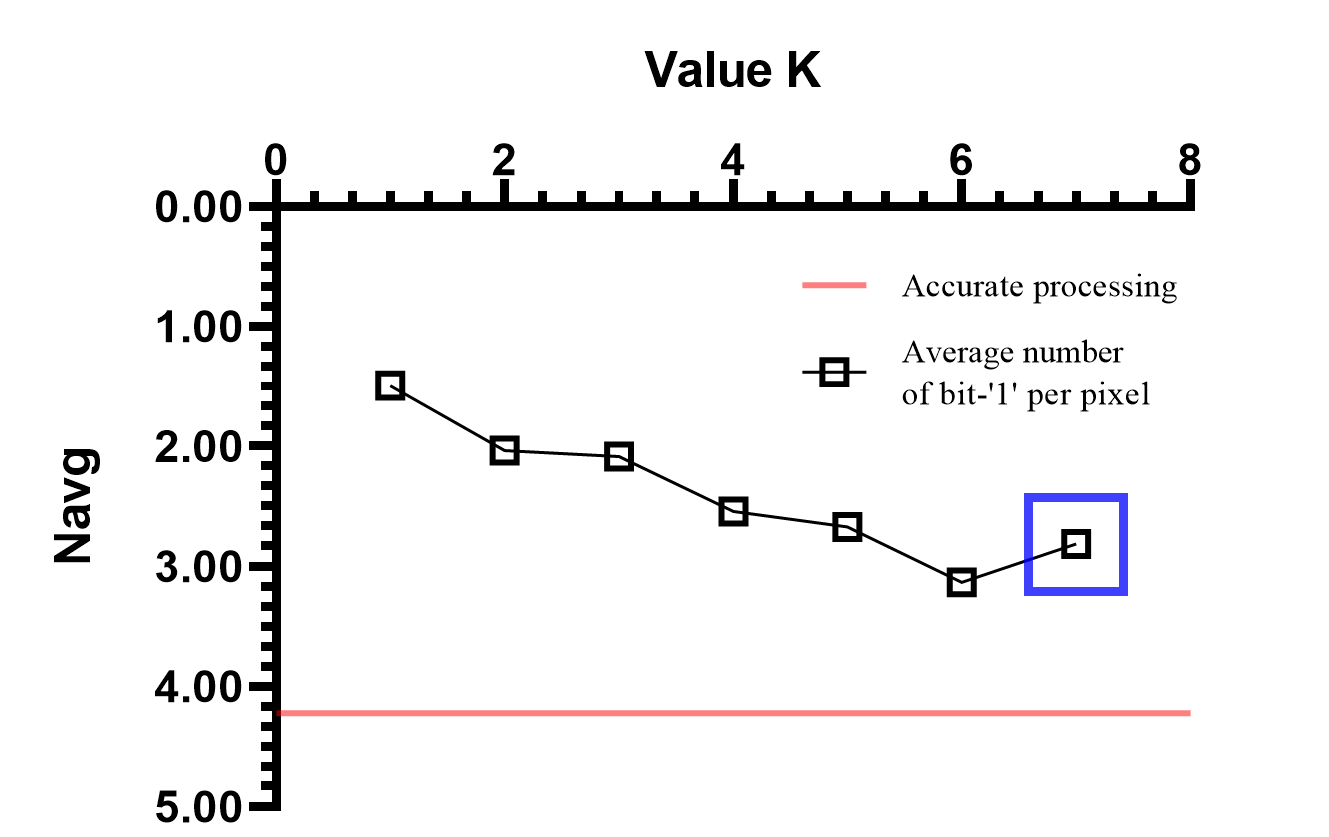
\includegraphics[width=\linewidth]{Fig/Average number of bit- `1' per pixel Navg for different value k.png}
\caption{Average number of bit- `1' per pixel Navg for different value $K$.}
\label{fig7}
\end{figure}

The image data is then sent to the SRAM model for further computation. Due to the high resolution of the image, it is not possible to send all of the data to the on-chip SRAM at once. As the capacity of the common SRAM is very limited and the size of SRAM affects the switch probability, two sizes of SRAM are used, which is 64k-bits and 128k-bits respectively. As shown in Fig. \ref{fig8}, the 128k-bits size SRAM has an overall significantly lower switch probability than that of 64k-bits size SRAM. The effect of distinct $K$ values on the switch probability is essentially the same as that of DRAM, where the switch probability for yet-to-be-preprocessed image data is close to 50\%, and decreases with smaller $K$ value. Thus, the storage power consumption of SRAM could be significantly reduced. However, this comes at the expense of output quality losses, and the following part will focus on the impact of image preprocessing on output quality.
\begin{figure}[htb]
\centering
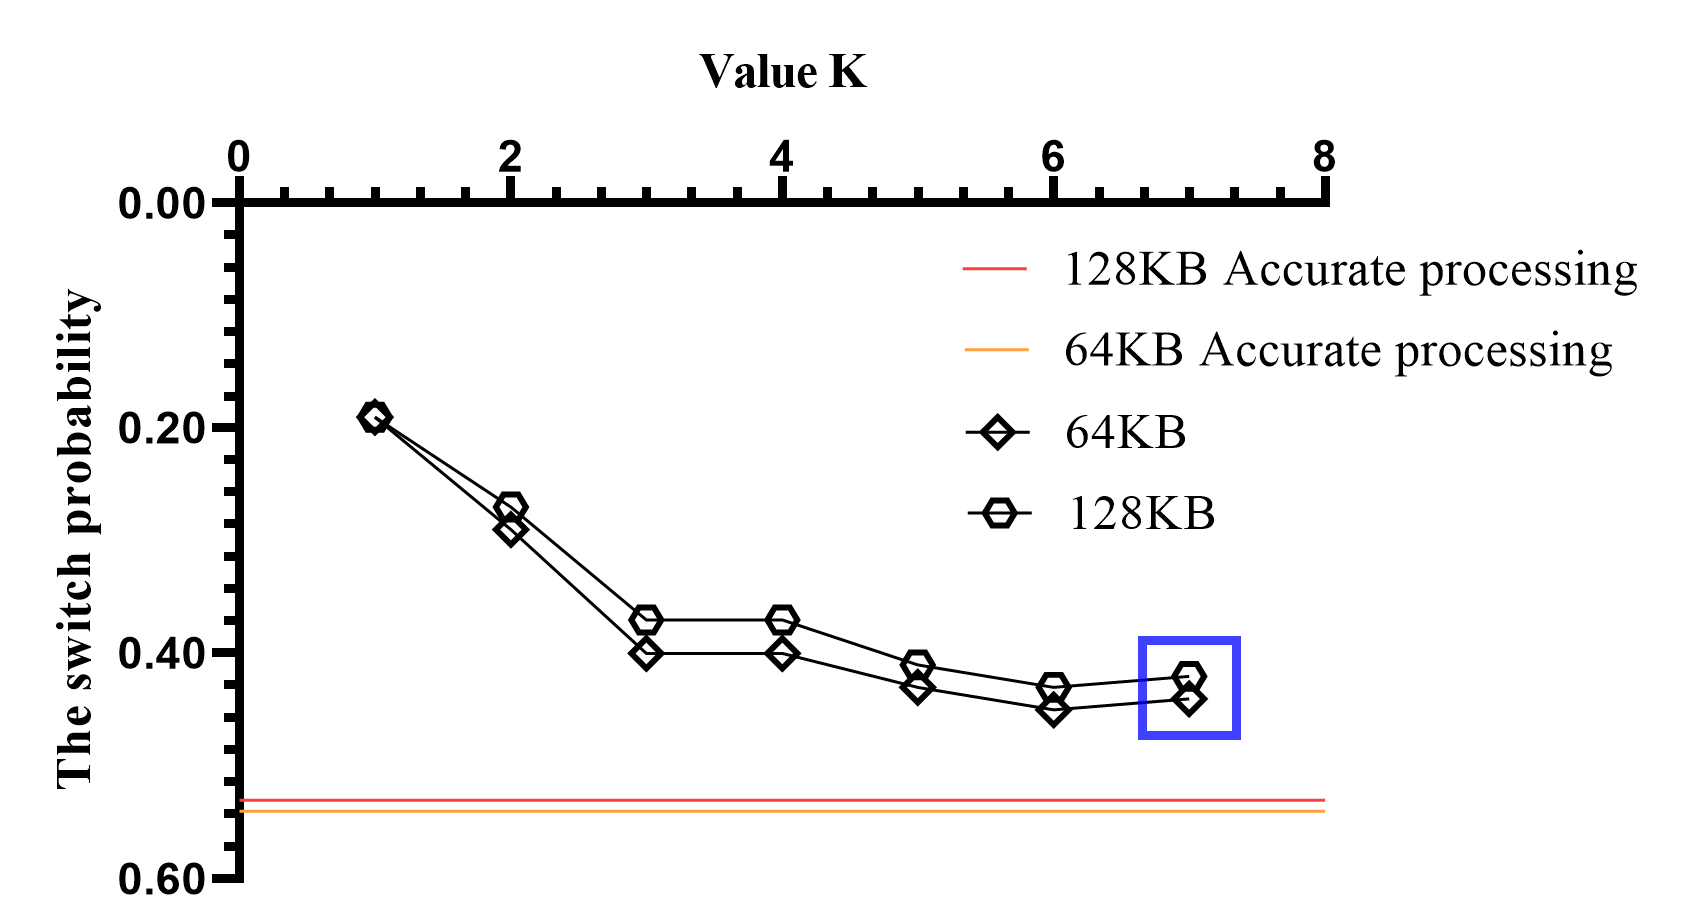
\includegraphics[width=\linewidth]{Fig/The switch probability for different value k.png}
\caption{The switch probability for different value $K$.}
\label{fig8}
\end{figure}

\subsection{The evaluation of output quality with the proposed strategy}
After analyzing the power consumption of DRAM and SRAM, the image data is processed with a decoder, which can be easily implemented into the integrated image processing algorithm. DCT, quantization, inverse quantization and IDCT in C++ are employed to process the approximated data after decoding. For the generality of the experimental results, 1 million images are used for the simulation. The final average PSNR with different $K$ values are shown in Fig. \ref{fig9}, where it can be seen that the output quality decreases with smaller $K$ value. Therefore, according to the requirements of different image applications, dynamic adjustment of off-chip and off-chip storage power consumption can be achieved based on output quality needs. When $K$ = 4, the proposed strategy in the paper has a\textcolor{red}{n average} PSNR loss of around 3.36 dB (compared to the accurate processing), and 39.8\% power reduction for DRAM and 25.9\% write power reduction for SRAM can be achieved. Additionally, as for the complete dropping method shown in Fig. 9, in which all the bits in the low part are set to be `0'. It can be seen that the complete dropping method has an overall significantly lower PSNR value than that of our proposed strategy. As the K decreases, the output quality decreases sharply, when $K$ = 4, the corresponding PSNR is \textcolor{red}{29.68}{\color{red}\sout{33.51}}dB, which {\color{red}\sout{means that 10\% reduction than our proposed strategy}}\textcolor{red}{is unacceptable in most practical applications}. This shows the effectiveness and efficiency of our approximation approach for error compensation. Fig. \ref{fig10} provides some examples \textcolor{red}{with proposed strategy.} \textcolor{red}{W}hen $K$ = 4, the appearance of the image processing are not significantly different from that of the accurate processing results. However, as $K$ increases, the PSNR value decreases and the image becomes substantially noisier.
\textcolor{red}{Fig. c shows the same examples with complete dropping method in order to prove the advantages of the proposed strategy in error compensation. The appearance of the image processing results is much more poor than that of the proposed strategy.}
\begin{figure}[htb]
	\centering
	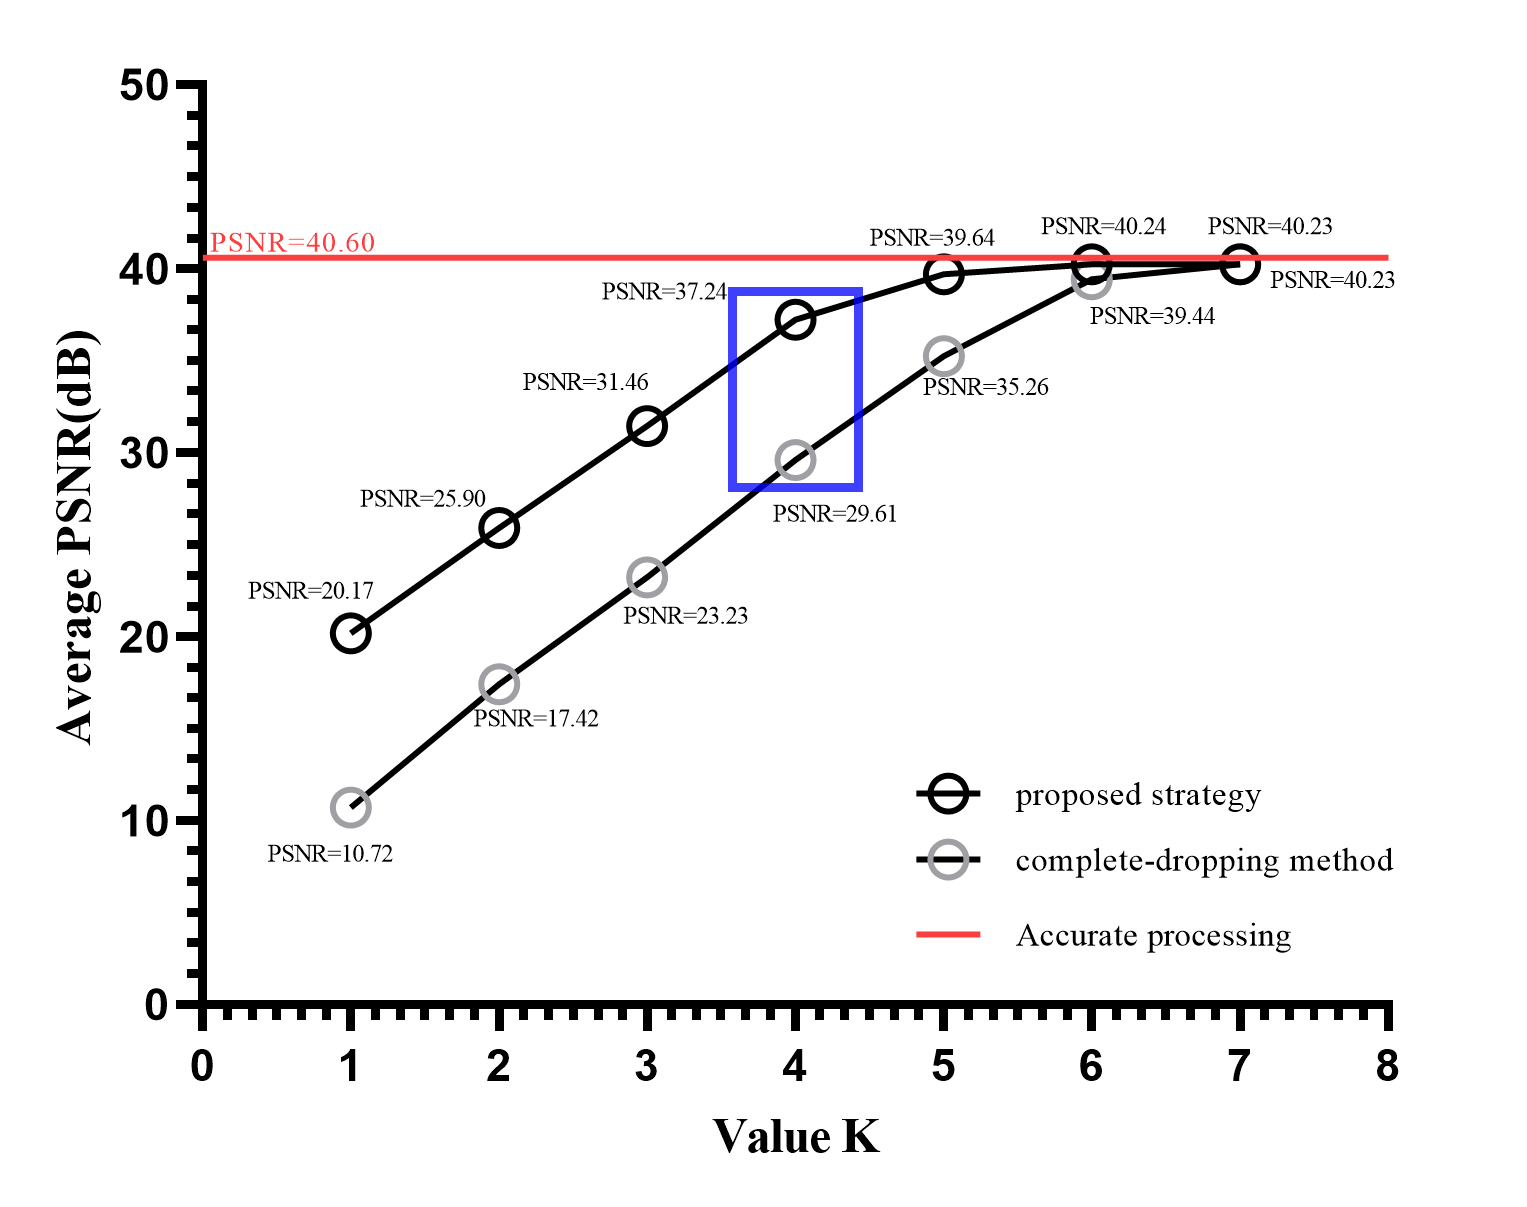
\includegraphics[width=\linewidth]{Fig/Average PSNR with different K value.png}
	\caption{Average PSNR with different value $K$.}
	\label{fig9}
\end{figure}
\begin{figure}[htb]
	\centering
	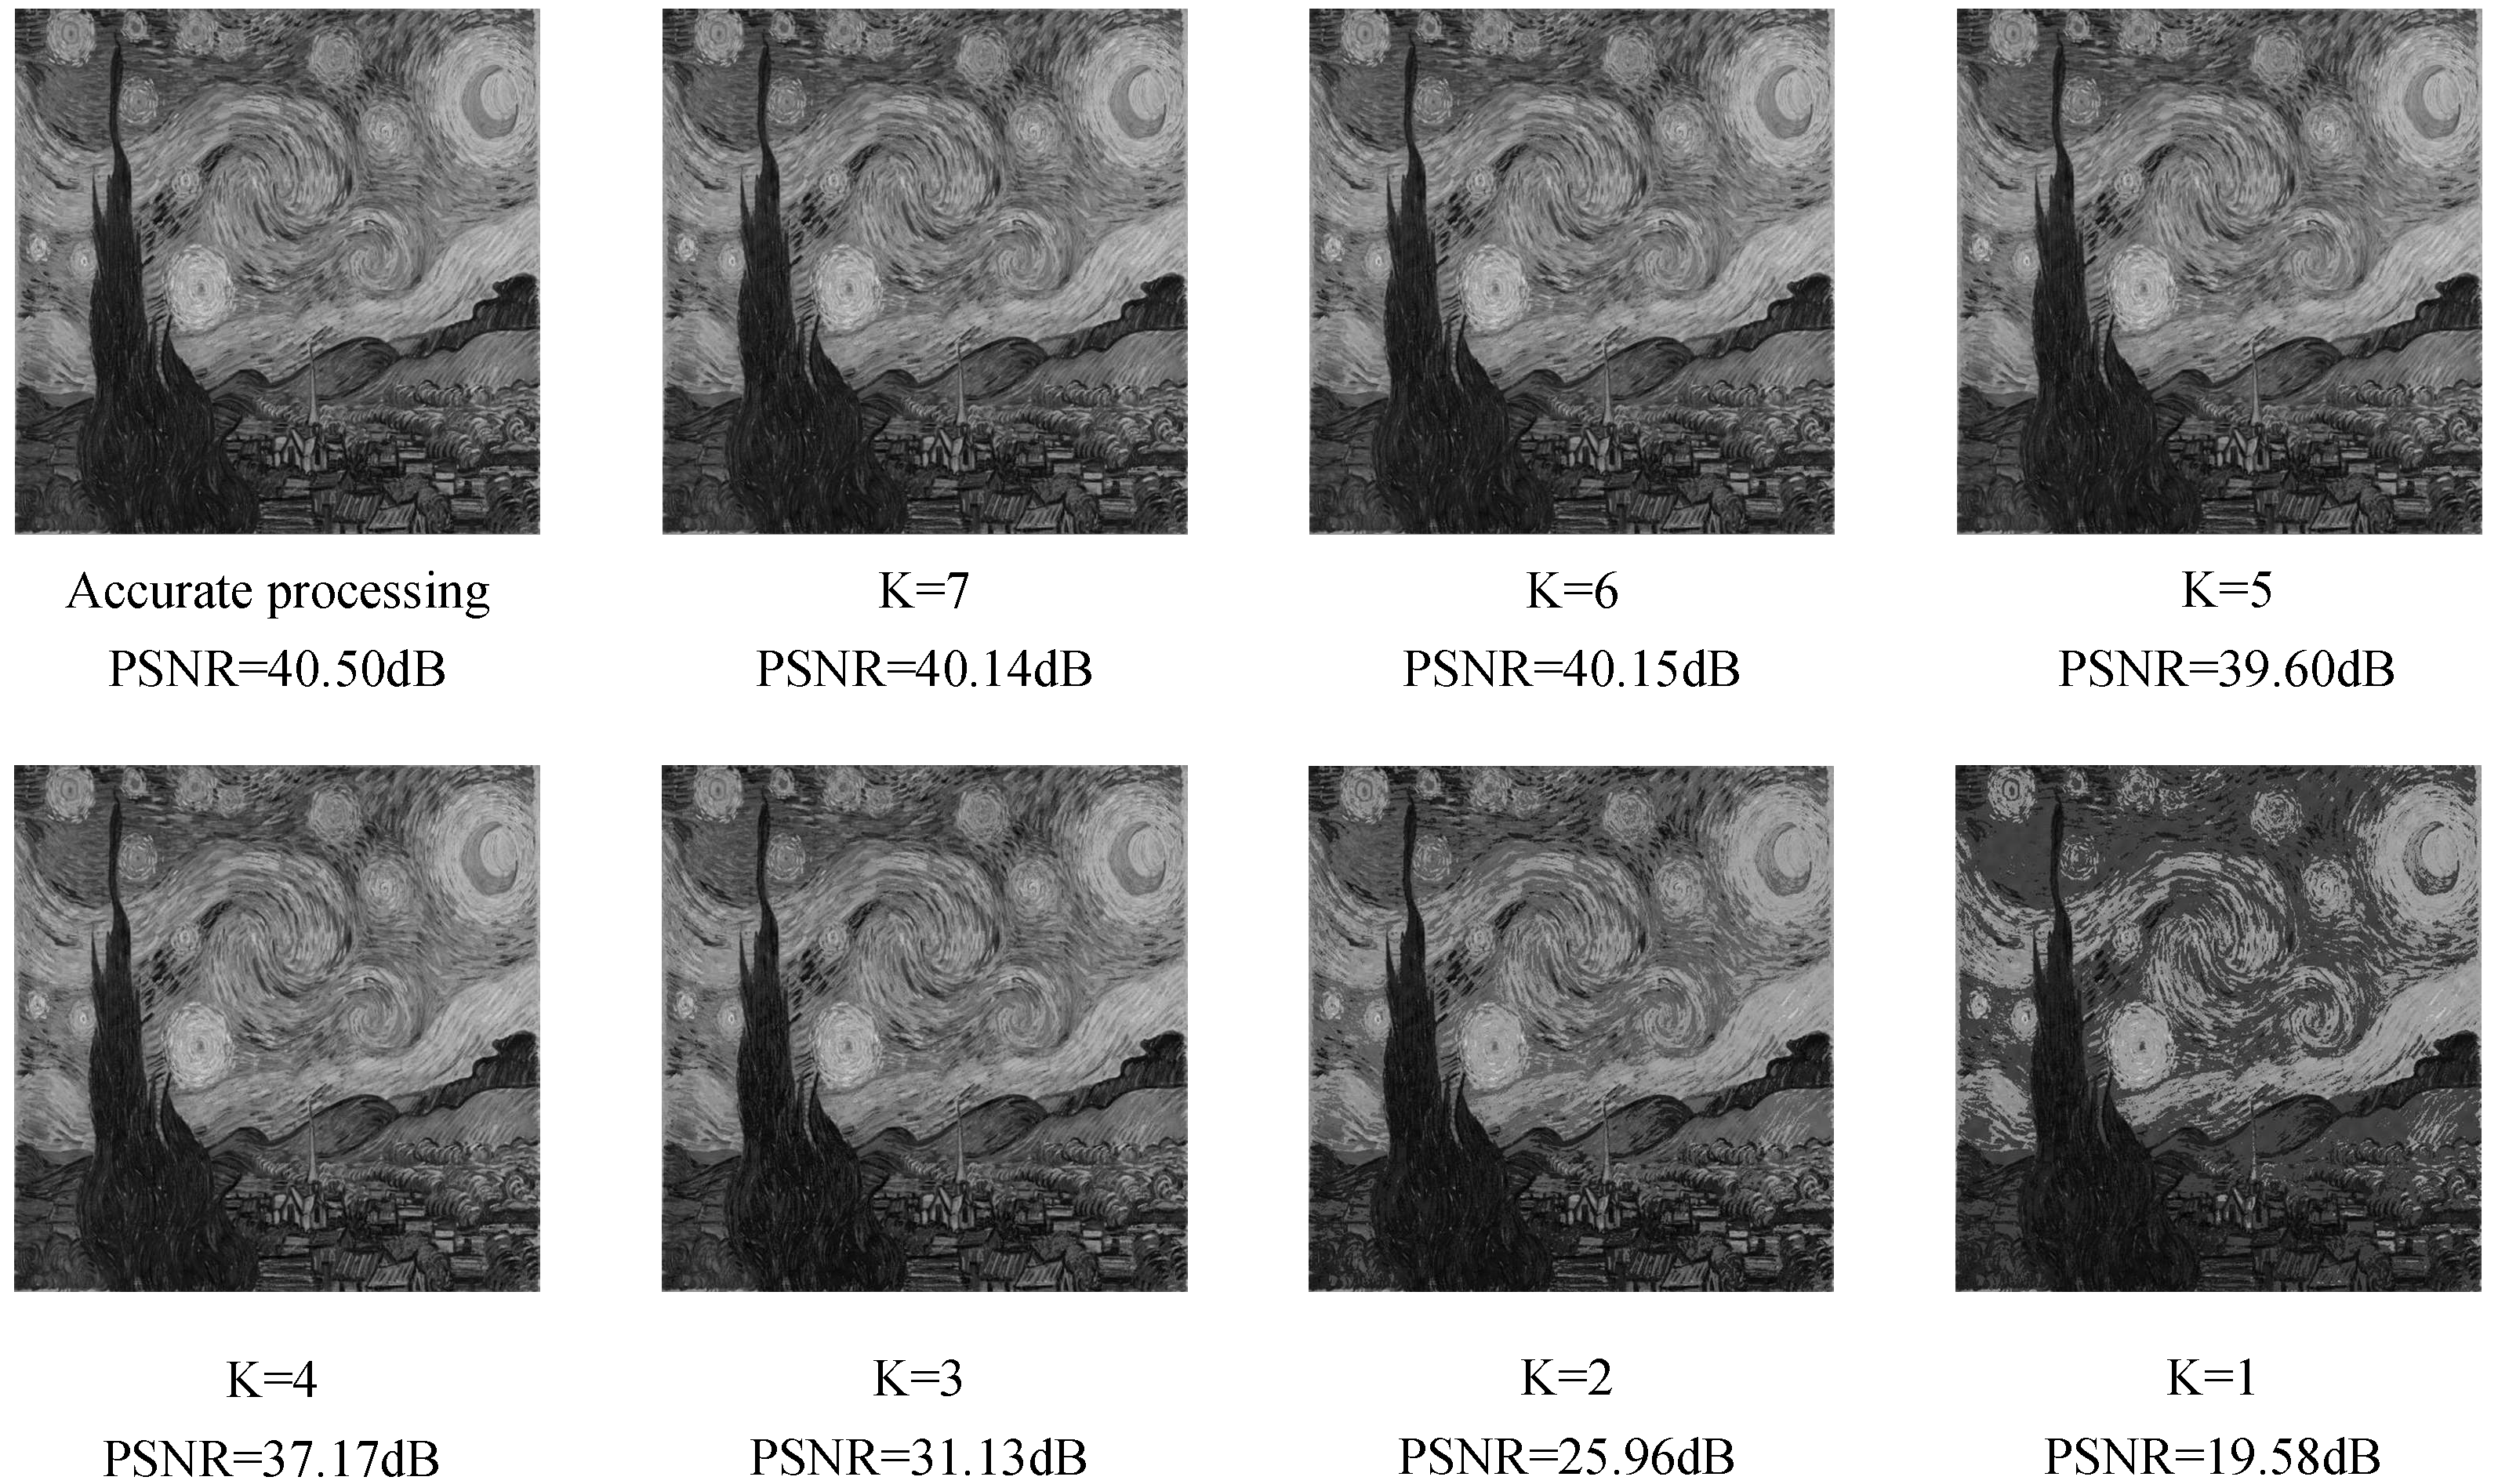
\includegraphics[width=\linewidth]{Fig/PSNR value of images with proposed strategy.png}
	\caption{PSNR value of images with proposed strategy.}
	\label{fig10}
\end{figure}


\subsection{The proposed strategy with a priority-based reduction in supply voltage}
According to Eq. \eqref{equ1}, the power consumption for SRAM is proportional to the supply voltage. As a result, lots of researches have been done in the past on reducing supply voltage for lower power dissipation. In this section, the proposed strategy is utilized jointly with an approximate mixed voltage storage scheme. More specifically, as shown in Fig. \ref{fig11}, the normal supply voltage is used for the accuracy of the high part as well as the flag bit, while the lower supply voltage is applied for the approximation of the low part. 
\begin{figure}[htb]
\centering
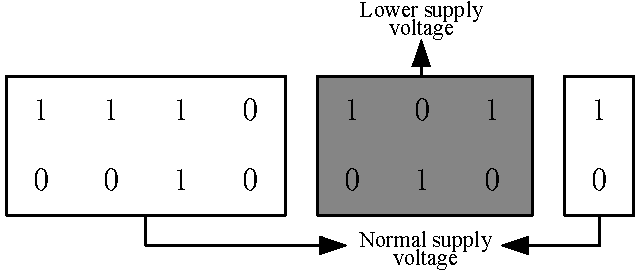
\includegraphics[width=\linewidth]{Fig/Selective reduction in supply voltage.png}
\caption{Selective reduction in supply voltage.}
\label{fig11}
\end{figure}

Theoretically, further reduction in power consumption for SRAM is attained. The evaluation of power saving can be expressed as follows:  
\begin{equation}
\label{equ2}
\boldsymbol{\eta }=\text{(}1-\boldsymbol{P}{{_{\mathrm{low}}}/{\boldsymbol{P}}}\text{)}*100\%
\end{equation}

Where $\boldsymbol{\eta}$ is the evaluation of power saving, $\boldsymbol{P}$ is the energy overhead with normal supply voltage, and $\boldsymbol{P_{\mathrm{low}}}$ is the energy overhead with selectively reduced supply voltage. In the case of $K$ = 4, the normal supply voltage is applied to the high part of 4 bits and the flag bit, while the lower supply voltage is applied to the low part of 3 bits. Thus, $\boldsymbol{P}$ and $\boldsymbol{P_{\mathrm{low}}}$ can be respectively replaced through Eq. \eqref{equ2}. Therefore, the evaluation of power saving can be calculated as follows:
$$
\boldsymbol{\eta }=[1-(\frac{5}{8}\boldsymbol{\alpha CV}_{\boldsymbol{DD}}^{2}\boldsymbol{f}+\frac{3}{8}\boldsymbol{\alpha CV}_{\mathrm{low}}^{2}\boldsymbol{f}{)/{\boldsymbol{\alpha }}}\boldsymbol{CV}_{\boldsymbol{DD}}^{2}\boldsymbol{f}]*100\% 
$$
\begin{equation}
\label{equ3} 
=(\frac{3}{8}-\frac{3}{8}\frac{\boldsymbol{V}_{\mathrm{low}}^{2}}{\boldsymbol{V}_{\boldsymbol{DD}}^{2}})*100\%
\end{equation}

Where $\boldsymbol{\eta}$  is the evaluation of power saving, $\boldsymbol{V_{DD}}$ is the normal supply voltage, while $\boldsymbol{V_{low}}$ is the lower supply voltage.
\begin{figure}[htb]
\centering
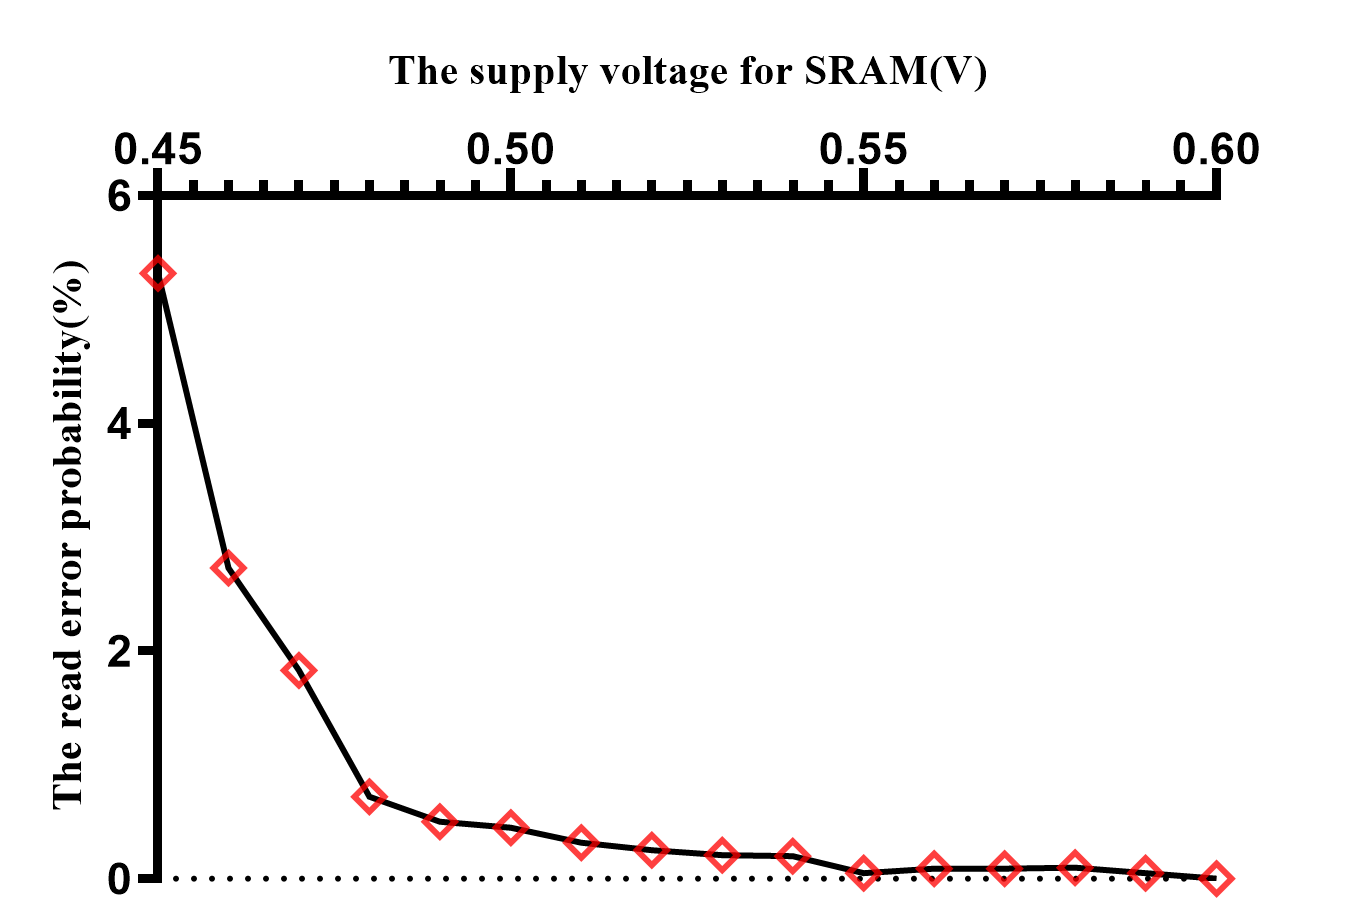
\includegraphics[width=\linewidth]{Fig/SRAM approximation error model.png}
\caption{SRAM approximation error model.}
\label{fig12}
\end{figure}

Undoubtedly, a lower supply voltage increases the probability of read errors from SRAM. Many researchers conducted in the past have presented the relationship between supply voltage and read error probability, as shown in Fig. \ref{fig12} \cite{9371622}. With lower supply voltage, the probability of read error increases. Hence, after the introduction of selectively reduction in supply voltage, a stochastic probability model is built in c++ to analyze the impact of selective reduced supply voltage on output quality. As shown in Table \ref{tab1}, the output quality PSNR does not decrease linearly with increasing read error probability; instead, an anti-correlation may occur. This is because some pixel information was lost during our approximation process, however, subsequent read errors may ``recover" the missing pixel information. Therefore, this strategy not only further reduces the storage power consumption, but also shows surprising results in terms of output quality.

{\color{red}\subsection{Discussion for hardware overhead}}
\textcolor{red}{In this section, the pre-processed circuit and the encoding circuit required for the methods proposed herein will be evaluated.} 

\textcolor{red}{For the pre-processing circuit used for the implementation of the data-compensated dropping method, the circuit structure under different approximate bit conditions is compiled by Verilog, and then synthesized by DesigningCompiler of Synopsys Company under SMIC65 nm process of SMIC Corp. The obtained gate-level netlist is sent to the PrimeTime Tool to acquire the data latency, power consumption, and area, which are regarded as the hardware overhead for discussion. From the analysis in section III, when $K=6$ and 7, the selective dropping method fails. Therefore, only the values of $K= 1,2,3,4,5$ are discussed herein. Furthermore, the additional power consumption of the added pre-processing circuit is low, and the area and latency increase are limited. Under the same conditions, when compared to the actual image and video encoding and decoding \cite{4342716}, the total power consumption of DRAM and SRAM is approximately 1W, and the areas of standard DRAM and 64k-bit SRAM are far greater than $\mu m^{2}$ -magnitude. Therefore, the power consumption and areas of the added circuits can be completely negligible in the actual system.}

\textcolor{red}{For the encoding algorithm, the hardware implementation cost of this method is displayed in Table II. It can be seen that the cost is only several hundred gates, which can be completely negligible in comparison with the MPEG-2 decoding system that requires nearly one million gates.}

\textcolor{red}{Compared the power consumption reduction with complete dropping method, like the simulation process in section IV. Navg in DRAM and the switch probability for SRAM based on the complete dropping method will also be evaluated. As can be seen in Table III, the complete dropping method gains more power reduction than the proposed strategy. However, according to the original intention of the designer, the output quality should be concerned with top priority. The output quality reduction for complete dropping strategy shown in Fig. 9 is significant, which cannot be accepted in most practical applications. Thus, the proposed strategy is more efficient and effective to achieve the tradeoff between output quality and storage power consumption.}


\begin{table} 
\begin{center} 
\caption{PSNR value of images with different supply voltage} 
\label{tab1} 
\begin{tabular}{| c | c | c |} 
\hline 
Supply voltage(V) & Read error probability(\%) & 
PSNR(dB)\\
\hline 
0.60& 0 
& 37.31\\ 
\hline
0.59& 0.05 
& 37.28\\
\hline 
0.58& 0.10 
& 37.27\\ 
\hline
0.57& 0.09
& 37.27\\ 
\hline
0.56& 0.09 
& 37.27\\ 
\hline
0.55& 0.05 
& 37.28\\ 
\hline
0.54& 0.20 
& 37.22\\ 
\hline
0.53& 0.21 
& 37.22\\ 
\hline
0.52& 0.25 
& 37.10\\ 
\hline
0.51& 0.32 
& 37.18\\ 
\hline
0.50& 0.45 
& 37.16\\ 
\hline
0.49& 0.50 
& 37.17\\ 
\hline
0.48& 0.72 
& 37.08\\ 
\hline
0.47& 1.83 
& 36.75\\ 
\hline
0.46& 2.73 
& 36.50\\ 
\hline
0.45& 5.32 
& 35.80\\ 
\hline
\end{tabular} 
\end{center} 
\end{table}
\section{Conclusion} \label{sec5}
In this paper, we presented a selective bit dropping and encoding co-strategy in image processing for low-power in DRAM and SRAM. Based on the characteristic of human visual system, the pixel data is selectively approximated and encoded in advance in order to provide a corresponding solution to reduce storage power consumption for both DRAM and SRAM, and the cost of the output quality and the system modification is negligible. The encoding strategy has shown its effectiveness and efficiency. At the same time, the selective bit dropping strategy archives the improvement on PSNR (compared to the complete dropping method). Our co-strategy decreases the number of bit-`1’ in original image data and contributes to the tradeoff between storage power consumption and output quality. More importantly, the approximate mixed voltage storage scheme has also been vertified its effectiveness and efficiency. Therefore, our co-strategy can be utilized in conjunction with other adaptive methods in the future work and we believe the proposed co-strategy could also provide the tradeoff between storage power consumption and output quality in various applications.


\bibliographystyle{IEEEtran}
\normalem\bibliography{reference}


\IEEEpubidadjcol
% Ibus el et quatemo luptatque doluptaest et pe volent rem ipidusa eribus utem venimolorae dera qui acea quam etur aceruptat.
% Gias anis doluptaspic tem et aliquis alique inctiuntiur?

% Sedigent, si aligend elibuscid ut et ium volo tem eictore pellore ritatus ut ut ullatus in con con pere nos ab ium di tem aliqui od magnit repta volectur suntio. Nam isquiante doluptis essit, ut eos suntionsecto debitiur sum ea ipitiis adipit, oditiore, a dolorerempos aut harum ius, atquat.

% Rum rem ditinti sciendunti volupiciendi sequiae nonsect oreniatur, volores sition ressimil inus solut ea volum harumqui to see\eqref{deqn_ex1a} mint aut quat eos explis ad quodi debis deliqui aspel earcius.

% \begin{equation}
% \label{deqn_ex1a}
% x = \sum_{i=0}^{n} 2{i} Q.
% \end{equation}

% Alis nime volorempera perferi sitio denim repudae pre ducilit atatet volecte ssimillorae dolore, ut pel ipsa nonsequiam in re nus maiost et que dolor sunt eturita tibusanis eatent a aut et dio blaudit reptibu scipitem liquia consequodi od unto ipsae. Et enitia vel et experferum quiat harum sa net faccae dolut voloria nem. Bus ut labo. Ita eum repraer rovitia samendit aut et volupta tecupti busant omni quiae porro que nossimodic temquis anto blacita conse nis am, que ereperum eumquam quaescil imenisci quae magnimos recus ilibeaque cum etum iliate prae parumquatemo blaceaquiam quundia dit apienditem rerit re eici quaes eos sinvers pelecabo. Namendignis as exerupit aut magnim ium illabor roratecte plic tem res apiscipsam et vernat untur a deliquaest que non cus eat ea dolupiducim fugiam volum hil ius dolo eaquis sitis aut landesto quo corerest et auditaquas ditae voloribus, qui optaspis exero cusa am, ut plibus.


% \section{Some Common Elements}
% \subsection{Sections and Subsections}
% Enumeration of section headings is desirable, but not required. When numbered, please be consistent throughout the article, that is, all headings and all levels of section headings in the article should be enumerated. Primary headings are designated with Roman numerals, secondary with capital letters, tertiary with Arabic numbers; and quaternary with lowercase letters. Reference and Acknowledgment headings are unlike all other section headings in text. They are never enumerated. They are simply primary headings without labels, regardless of whether the other headings in the article are enumerated. 

% \subsection{Citations to the Bibliography}
% The coding for the citations is made with the \LaTeX\ $\backslash${\tt{cite}} command. 
% This will display as: see \cite{ref1}.

% For multiple citations code as follows: {\tt{$\backslash$cite\{ref1,ref2,ref3\}}}
%  which will produce \cite{ref1,ref2,ref3}. For reference ranges that are not consecutive code as {\tt{$\backslash$cite\{ref1,ref2,ref3,ref9\}}} which will produce  \cite{ref1,ref2,ref3,ref9}

% \subsection{Lists}
% In this section, we will consider three types of lists: simple unnumbered, numbered, and bulleted. There have been many options added to IEEEtran to enhance the creation of lists. If your lists are more complex than those shown below, please refer to the original ``IEEEtran\_HOWTO.pdf'' for additional options.\\

% \subsubsection*{\bf A plain  unnumbered list}
% \begin{list}{}{}
% \item{bare\_jrnl.tex}
% \item{bare\_conf.tex}
% \item{bare\_jrnl\_compsoc.tex}
% \item{bare\_conf\_compsoc.tex}
% \item{bare\_jrnl\_comsoc.tex}
% \end{list}

% \subsubsection*{\bf A simple numbered list}
% \begin{enumerate}
% \item{bare\_jrnl.tex}
% \item{bare\_conf.tex}
% \item{bare\_jrnl\_compsoc.tex}
% \item{bare\_conf\_compsoc.tex}
% \item{bare\_jrnl\_comsoc.tex}
% \end{enumerate}

% \subsubsection*{\bf A simple bulleted list}
% \begin{itemize}
% \item{bare\_jrnl.tex}
% \item{bare\_conf.tex}
% \item{bare\_jrnl\_compsoc.tex}
% \item{bare\_conf\_compsoc.tex}
% \item{bare\_jrnl\_comsoc.tex}
% \end{itemize}





% \subsection{Figures}
% Fig. 1 is an example of a floating figure using the graphicx package.
%  Note that $\backslash${\tt{label}} must occur AFTER (or within) $\backslash${\tt{caption}}.
%  For figures, $\backslash${\tt{caption}} should occur after the $\backslash${\tt{includegraphics}}.

% \begin{figure}[!t]
% \centering
% \includegraphics[width=2.5in]{fig1}
% \caption{Simulation results for the network.}
% \label{fig_1}
% \end{figure}

% Fig. 2(a) and 2(b) is an example of a double column floating figure using two subfigures.
%  (The subfig.sty package must be loaded for this to work.)
%  The subfigure $\backslash${\tt{label}} commands are set within each subfloat command,
%  and the $\backslash${\tt{label}} for the overall figure must come after $\backslash${\tt{caption}}.
%  $\backslash${\tt{hfil}} is used as a separator to get equal spacing.
%  The combined width of all the parts of the figure should do not exceed the text width or a line break will occur.
% %
% \begin{figure*}[!t]
% \centering
% \subfloat[]{\includegraphics[width=2.5in]{fig1}%
% \label{fig_first_case}}
% \hfil
% \subfloat[]{\includegraphics[width=2.5in]{fig1}%
% \label{fig_second_case}}
% \caption{Dae. Ad quatur autat ut porepel itemoles dolor autem fuga. Bus quia con nessunti as remo di quatus non perum que nimus. (a) Case I. (b) Case II.}
% \label{fig_sim}
% \end{figure*}

% Note that often IEEE papers with multi-part figures do not place the labels within the image itself (using the optional argument to $\backslash${\tt{subfloat}}[]), but instead will
%  reference/describe all of them (a), (b), etc., within the main caption.
%  Be aware that for subfig.sty to generate the (a), (b), etc., subfigure
%  labels, the optional argument to $\backslash${\tt{subfloat}} must be present. If a
%  subcaption is not desired, leave its contents blank,
%  e.g.,$\backslash${\tt{subfloat}}[].


 

% \section{Tables}
% Note that, for IEEE-style tables, the
%  $\backslash${\tt{caption}} command should come BEFORE the table. Table captions use title case. Articles (a, an, the), coordinating conjunctions (and, but, for, or, nor), and most short prepositions are lowercase unless they are the first or last word. Table text will default to $\backslash${\tt{footnotesize}} as
%  the IEEE normally uses this smaller font for tables.
%  The $\backslash${\tt{label}} must come after $\backslash${\tt{caption}} as always.
 
% \begin{table}[!t]
% \caption{An Example of a Table\label{tab:table1}}
% \centering
% \begin{tabular}{|c||c|}
% \hline
% One & Two\\
% \hline
% Three & Four\\
% \hline
% \end{tabular}
% \end{table}

% \section{Algorithms}
% Algorithms should be numbered and include a short title. They are set off from the text with rules above and below the title and after the last line.

% \begin{algorithm}[H]
% \caption{Weighted Tanimoto ELM.}\label{alg:alg1}
% \begin{algorithmic}
% \STATE 
% \STATE {\textsc{TRAIN}}$(\mathbf{X} \mathbf{T})$
% \STATE \hspace{0.5cm}$ \textbf{select randomly } W \subset \mathbf{X}  $
% \STATE \hspace{0.5cm}$ N_\mathbf{t} \gets | \{ i : \mathbf{t}_i = \mathbf{t} \} | $ \textbf{ for } $ \mathbf{t}= -1,+1 $
% \STATE \hspace{0.5cm}$ B_i \gets \sqrt{ \textsc{max}(N_{-1},N_{+1}) / N_{\mathbf{t}_i} } $ \textbf{ for } $ i = 1,...,N $
% \STATE \hspace{0.5cm}$ \hat{\mathbf{H}} \gets  B \cdot (\mathbf{X}^T\textbf{W})/( \mathbb{1}\mathbf{X} + \mathbb{1}\textbf{W} - \mathbf{X}^T\textbf{W} ) $
% \STATE \hspace{0.5cm}$ \beta \gets \left ( I/C + \hat{\mathbf{H}}^T\hat{\mathbf{H}} \right )^{-1}(\hat{\mathbf{H}}^T B\cdot \mathbf{T})  $
% \STATE \hspace{0.5cm}\textbf{return}  $\textbf{W},  \beta $
% \STATE 
% \STATE {\textsc{PREDICT}}$(\mathbf{X} )$
% \STATE \hspace{0.5cm}$ \mathbf{H} \gets  (\mathbf{X}^T\textbf{W} )/( \mathbb{1}\mathbf{X}  + \mathbb{1}\textbf{W}- \mathbf{X}^T\textbf{W}  ) $
% \STATE \hspace{0.5cm}\textbf{return}  $\textsc{sign}( \mathbf{H} \beta )$
% \end{algorithmic}
% \label{alg1}
% \end{algorithm}

% Que sunt eum lam eos si dic to estist, culluptium quid qui nestrum nobis reiumquiatur minimus minctem. Ro moluptat fuga. Itatquiam ut laborpo rersped exceres vollandi repudaerem. Ulparci sunt, qui doluptaquis sumquia ndestiu sapient iorepella sunti veribus. Ro moluptat fuga. Itatquiam ut laborpo rersped exceres vollandi repudaerem. 
% \section{Mathematical Typography \\ and Why It Matters}

% Typographical conventions for mathematical formulas have been developed to {\bf provide uniformity and clarity of presentation across mathematical texts}. This enables the readers of those texts to both understand the author's ideas and to grasp new concepts quickly. While software such as \LaTeX \ and MathType\textsuperscript{\textregistered} can produce aesthetically pleasing math when used properly, it is also very easy to misuse the software, potentially resulting in incorrect math display.

% IEEE aims to provide authors with the proper guidance on mathematical typesetting style and assist them in writing the best possible article. As such, IEEE has assembled a set of examples of good and bad mathematical typesetting \cite{ref1,ref2,ref3,ref4,ref5}. 

% Further examples can be found at \url{http://journals.ieeeauthorcenter.ieee.org/wp-content/uploads/sites/7/IEEE-Math-Typesetting-Guide-for-LaTeX-Users.pdf}

% \subsection{Display Equations}
% The simple display equation example shown below uses the ``equation'' environment. To number the equations, use the $\backslash${\tt{label}} macro to create an identifier for the equation. LaTeX will automatically number the equation for you.
% \begin{equation}
% \label{deqn_ex1}
% x = \sum_{i=0}^{n} 2{i} Q.
% \end{equation}

% \noindent is coded as follows:
% \begin{verbatim}
% \begin{equation}
% \label{deqn_ex1}
% x = \sum_{i=0}^{n} 2{i} Q.
% \end{equation}
% \end{verbatim}

% To reference this equation in the text use the $\backslash${\tt{ref}} macro. 
% Please see (\ref{deqn_ex1})\\
% \noindent is coded as follows:
% \begin{verbatim}
% Please see (\ref{deqn_ex1})\end{verbatim}

% \subsection{Equation Numbering}
% {\bf{Consecutive Numbering:}} Equations within an article are numbered consecutively from the beginning of the
% article to the end, i.e., (1), (2), (3), (4), (5), etc. Do not use roman numerals or section numbers for equation numbering.

% \noindent {\bf{Appendix Equations:}} The continuation of consecutively numbered equations is best in the Appendix, but numbering
%  as (A1), (A2), etc., is permissible.\\

% \noindent {\bf{Hyphens and Periods}}: Hyphens and periods should not be used in equation numbers, i.e., use (1a) rather than
% (1-a) and (2a) rather than (2.a) for subequations. This should be consistent throughout the article.

% \subsection{Multi-Line Equations and Alignment}
% Here we show several examples of multi-line equations and proper alignments.

% \noindent {\bf{A single equation that must break over multiple lines due to length with no specific alignment.}}
% \begin{multline}
% \text{The first line of this example}\\
% \text{The second line of this example}\\
% \text{The third line of this example}
% \end{multline}

% \noindent is coded as:
% \begin{verbatim}
% \begin{multline}
% \text{The first line of this example}\\
% \text{The second line of this example}\\
% \text{The third line of this example}
% \end{multline}
% \end{verbatim}

% \noindent {\bf{A single equation with multiple lines aligned at the = signs}}
% \begin{align}
% a &= c+d \\
% b &= e+f
% \end{align}
% \noindent is coded as:
% \begin{verbatim}
% \begin{align}
% a &= c+d \\
% b &= e+f
% \end{align}
% \end{verbatim}

% The {\tt{align}} environment can align on multiple  points as shown in the following example:
% \begin{align}
% x &= y & X & =Y & a &=bc\\
% x' &= y' & X' &=Y' &a' &=bz
% \end{align}
% \noindent is coded as:
% \begin{verbatim}
% \begin{align}
% x &= y & X & =Y & a &=bc\\
% x' &= y' & X' &=Y' &a' &=bz
% \end{align}
% \end{verbatim}





% \subsection{Subnumbering}
% The amsmath package provides a {\tt{subequations}} environment to facilitate subnumbering. An example:

% \begin{subequations}\label{eq:2}
% \begin{align}
% f&=g \label{eq:2A}\\
% f' &=g' \label{eq:2B}\\
% \mathcal{L}f &= \mathcal{L}g \label{eq:2c}
% \end{align}
% \end{subequations}

% \noindent is coded as:
% \begin{verbatim}
% \begin{subequations}\label{eq:2}
% \begin{align}
% f&=g \label{eq:2A}\\
% f' &=g' \label{eq:2B}\\
% \mathcal{L}f &= \mathcal{L}g \label{eq:2c}
% \end{align}
% \end{subequations}

% \end{verbatim}

% \subsection{Matrices}
% There are several useful matrix environments that can save you some keystrokes. See the example coding below and the output.

% \noindent {\bf{A simple matrix:}}
% \begin{equation}
% \begin{matrix}  0 &  1 \\ 
% 1 &  0 \end{matrix}
% \end{equation}
% is coded as:
% \begin{verbatim}
% \begin{equation}
% \begin{matrix}  0 &  1 \\ 
% 1 &  0 \end{matrix}
% \end{equation}
% \end{verbatim}

% \noindent {\bf{A matrix with parenthesis}}
% \begin{equation}
% \begin{pmatrix} 0 & -i \\
%  i &  0 \end{pmatrix}
% \end{equation}
% is coded as:
% \begin{verbatim}
% \begin{equation}
% \begin{pmatrix} 0 & -i \\
%  i &  0 \end{pmatrix}
% \end{equation}
% \end{verbatim}

% \noindent {\bf{A matrix with square brackets}}
% \begin{equation}
% \begin{bmatrix} 0 & -1 \\ 
% 1 &  0 \end{bmatrix}
% \end{equation}
% is coded as:
% \begin{verbatim}
% \begin{equation}
% \begin{bmatrix} 0 & -1 \\ 
% 1 &  0 \end{bmatrix}
% \end{equation}
% \end{verbatim}

% \noindent {\bf{A matrix with curly braces}}
% \begin{equation}
% \begin{Bmatrix} 1 &  0 \\ 
% 0 & -1 \end{Bmatrix}
% \end{equation}
% is coded as:
% \begin{verbatim}
% \begin{equation}
% \begin{Bmatrix} 1 &  0 \\ 
% 0 & -1 \end{Bmatrix}
% \end{equation}\end{verbatim}

% \noindent {\bf{A matrix with single verticals}}
% \begin{equation}
% \begin{vmatrix} a &  b \\ 
% c &  d \end{vmatrix}
% \end{equation}
% is coded as:
% \begin{verbatim}
% \begin{equation}
% \begin{vmatrix} a &  b \\ 
% c &  d \end{vmatrix}
% \end{equation}\end{verbatim}

% \noindent {\bf{A matrix with double verticals}}
% \begin{equation}
% \begin{Vmatrix} i &  0 \\ 
% 0 & -i \end{Vmatrix}
% \end{equation}
% is coded as:
% \begin{verbatim}
% \begin{equation}
% \begin{Vmatrix} i &  0 \\ 
% 0 & -i \end{Vmatrix}
% \end{equation}\end{verbatim}

% \subsection{Arrays}
% The {\tt{array}} environment allows you some options for matrix-like equations. You will have to manually key the fences, but there are other options for alignment of the columns and for setting horizontal and vertical rules. The argument to {\tt{array}} controls alignment and placement of vertical rules.

% A simple array
% \begin{equation}
% \left(
% \begin{array}{cccc}
% a+b+c & uv & x-y & 27\\
% a+b & u+v & z & 134
% \end{array}\right)
% \end{equation}
% is coded as:
% \begin{verbatim}
% \begin{equation}
% \left(
% \begin{array}{cccc}
% a+b+c & uv & x-y & 27\\
% a+b & u+v & z & 134
% \end{array} \right)
% \end{equation}
% \end{verbatim}

% A slight variation on this to better align the numbers in the last column
% \begin{equation}
% \left(
% \begin{array}{cccr}
% a+b+c & uv & x-y & 27\\
% a+b & u+v & z & 134
% \end{array}\right)
% \end{equation}
% is coded as:
% \begin{verbatim}
% \begin{equation}
% \left(
% \begin{array}{cccr}
% a+b+c & uv & x-y & 27\\
% a+b & u+v & z & 134
% \end{array} \right)
% \end{equation}
% \end{verbatim}

% An array with vertical and horizontal rules
% \begin{equation}
% \left( \begin{array}{c|c|c|r}
% a+b+c & uv & x-y & 27\\ \hline
% a+b & u+v & z & 134
% \end{array}\right)
% \end{equation}
% is coded as:
% \begin{verbatim}
% \begin{equation}
% \left(
% \begin{array}{c|c|c|r}
% a+b+c & uv & x-y & 27\\
% a+b & u+v & z & 134
% \end{array} \right)
% \end{equation}
% \end{verbatim}
% Note the argument now has the pipe "$\vert$" included to indicate the placement of the vertical rules.


% \subsection{Cases Structures}
% Many times cases can be miscoded using the wrong environment, i.e., {\tt{array}}. Using the {\tt{cases}} environment will save keystrokes (from not having to type the $\backslash${\tt{left}}$\backslash${\tt{lbrace}}) and automatically provide the correct column alignment.
% \begin{equation*}
% {z_m(t)} = \begin{cases}
% 1,&{\text{if}}\ {\beta }_m(t) \\ 
% {0,}&{\text{otherwise.}} 
% \end{cases}
% \end{equation*}
% \noindent is coded as follows:
% \begin{verbatim}
% \begin{equation*}
% {z_m(t)} = 
% \begin{cases}
% 1,&{\text{if}}\ {\beta }_m(t),\\ 
% {0,}&{\text{otherwise.}} 
% \end{cases}
% \end{equation*}
% \end{verbatim}
% \noindent Note that the ``\&'' is used to mark the tabular alignment. This is important to get  proper column alignment. Do not use $\backslash${\tt{quad}} or other fixed spaces to try and align the columns. Also, note the use of the $\backslash${\tt{text}} macro for text elements such as ``if'' and ``otherwise.''

% \subsection{Function Formatting in Equations}
% Often, there is an easy way to properly format most common functions. Use of the $\backslash$ in front of the function name will in most cases, provide the correct formatting. When this does not work, the following example provides a solution using the $\backslash${\tt{text}} macro:

% \begin{equation*} 
%   d_{R}^{KM} = \underset {d_{l}^{KM}} {\text{arg min}} \{ d_{1}^{KM},\ldots,d_{6}^{KM}\}.
% \end{equation*}

% \noindent is coded as follows:
% \begin{verbatim}
% \begin{equation*} 
%  d_{R}^{KM} = \underset {d_{l}^{KM}} 
%  {\text{arg min}} \{ d_{1}^{KM},
%  \ldots,d_{6}^{KM}\}.
% \end{equation*}
% \end{verbatim}

% \subsection{ Text Acronyms Inside Equations}
% This example shows where the acronym ``MSE" is coded using $\backslash${\tt{text\{\}}} to match how it appears in the text.

% \begin{equation*}
%  \text{MSE} = \frac {1}{n}\sum _{i=1}^{n}(Y_{i} - \hat {Y_{i}})^{2}
% \end{equation*}

% \begin{verbatim}
% \begin{equation*}
%  \text{MSE} = \frac {1}{n}\sum _{i=1}^{n}
% (Y_{i} - \hat {Y_{i}})^{2}
% \end{equation*}
% \end{verbatim}

% \section{Conclusion}
% The conclusion goes here.


% \section*{Acknowledgments}
% This should be a simple paragraph before the References to thank those individuals and institutions who have supported your work on this article.



% {\appendix[Proof of the Zonklar Equations]
% Use $\backslash${\tt{appendix}} if you have a single appendix:
% Do not use $\backslash${\tt{section}} anymore after $\backslash${\tt{appendix}}, only $\backslash${\tt{section*}}.
% If you have multiple appendixes use $\backslash${\tt{appendices}} then use $\backslash${\tt{section}} to start each appendix.
% You must declare a $\backslash${\tt{section}} before using any $\backslash${\tt{subsection}} or using $\backslash${\tt{label}} ($\backslash${\tt{appendices}} by itself
%  starts a section numbered zero.)}



% %{\appendices
% %\section*{Proof of the First Zonklar Equation}
% %Appendix one text goes here.
% % You can choose not to have a title for an appendix if you want by leaving the argument blank
% %\section*{Proof of the Second Zonklar Equation}
% %Appendix two text goes here.}



% \section{References Section}
% You can use a bibliography generated by BibTeX as a .bbl file.
%  BibTeX documentation can be easily obtained at:
%  http://mirror.ctan.org/biblio/bibtex/contrib/doc/
%  The IEEEtran BibTeX style support page is:
%  http://www.michaelshell.org/tex/ieeetran/bibtex/



%  % argument is your BibTeX string definitions and bibliography database(s)
% %\bibliography{IEEEabrv,../bib/paper}
% %
% \section{Simple References}
% You can manually copy in the resultant .bbl file and set second argument of $\backslash${\tt{begin}} to the number of references
%  (used to reserve space for the reference number labels box).

% \begin{thebibliography}{1}
% \bibliographystyle{IEEEtran}

% \bibitem{ref1}
% {\it{Mathematics Into Type}}. American Mathematical Society. [Online]. Available: https://www.ams.org/arc/styleguide/mit-2.pdf

% \bibitem{ref2}
% T. W. Chaundy, P. R. Barrett and C. Batey, {\it{The Printing of Mathematics}}. London, U.K., Oxford Univ. Press, 1954.

% \bibitem{ref3}
% F. Mittelbach and M. Goossens, {\it{The \LaTeX Companion}}, 2nd ed. Boston, MA, USA: Pearson, 2004.

% \bibitem{ref4}
% G. Gr\"atzer, {\it{More Math Into LaTeX}}, New York, NY, USA: Springer, 2007.

% \bibitem{ref5}M. Letourneau and J. W. Sharp, {\it{AMS-StyleGuide-online.pdf,}} American Mathematical Society, Providence, RI, USA, [Online]. Available: http://www.ams.org/arc/styleguide/index.html

% \bibitem{ref6}
% H. Sira-Ramirez, ``On the sliding mode control of nonlinear systems,'' \textit{Syst. Control Lett.}, vol. 19, pp. 303--312, 1992.

% \bibitem{ref7}
% A. Levant, ``Exact differentiation of signals with unbounded higher derivatives,''  in \textit{Proc. 45th IEEE Conf. Decis.
% Control}, San Diego, CA, USA, 2006, pp. 5585--5590. DOI: 10.1109/CDC.2006.377165.

% \bibitem{ref8}
% M. Fliess, C. Join, and H. Sira-Ramirez, ``Non-linear estimation is easy,'' \textit{Int. J. Model., Ident. Control}, vol. 4, no. 1, pp. 12--27, 2008.

% \bibitem{ref9}
% R. Ortega, A. Astolfi, G. Bastin, and H. Rodriguez, ``Stabilization of food-chain systems using a port-controlled Hamiltonian description,'' in \textit{Proc. Amer. Control Conf.}, Chicago, IL, USA,
% 2000, pp. 2245--2249.

% \end{thebibliography}


% \newpage

% \section{Biography Section}
% If you have an EPS/PDF photo (graphicx package needed), extra braces are
%  needed around the contents of the optional argument to biography to prevent
%  the LaTeX parser from getting confused when it sees the complicated
%  $\backslash${\tt{includegraphics}} command within an optional argument. (You can create
%  your own custom macro containing the $\backslash${\tt{includegraphics}} command to make things
%  simpler here.)
 
% \vspace{11pt}

% \bf{If you include a photo:}\vspace{-33pt}
% \begin{IEEEbiography}[{\includegraphics[width=1in,height=1.25in,clip,keepaspectratio]{fig1}}]{Michael Shell}
% Use $\backslash${\tt{begin\{IEEEbiography\}}} and then for the 1st argument use $\backslash${\tt{includegraphics}} to declare and link the author photo.
% Use the author name as the 3rd argument followed by the biography text.
% \end{IEEEbiography}

% \vspace{11pt}

% \bf{If you will not include a photo:}\vspace{-33pt}
% \begin{IEEEbiographynophoto}{John Doe}
% Use $\backslash${\tt{begin\{IEEEbiographynophoto\}}} and the author name as the argument followed by the biography text.
% \end{IEEEbiographynophoto}




\vfill

\end{document}


